% !TeX program = xelatex
% ============================================================
% 1999 年·普通高等学校招生全国统一考试·广东卷 · 解析版
% 由 tools/make_editions.py 生成（重跑会覆盖本文件）；
% 题目/解析内容在 questions.tex / answers*.tex，勿在本文件内写内容。
% ============================================================
\documentclass[zihao=-4, a4paper]{ctexart}
% ============================================================
% common/preamble.tex —— 拆分版试卷项目 · 公共导言区
% 引擎：XeLaTeX；文档类 ctexart 由各版本壳文件自行声明
% 由合并书 math-gaokao-2017-2026/preamble.tex 改造而来：
%   - 页眉左右改为可重定义宏 \gkheadL / \gkheadR（各版本壳设置）
%   - hyperref 不再写死 pdftitle（壳内 \hypersetup 覆盖）
%   - 删除书籍专用的 \chaptermark 重定义与 \gkpaper 装配宏
% ============================================================

% ---------- 数学 ----------
\usepackage{amsmath}
\usepackage{amssymb}
\usepackage{mathtools}

% ---------- 绘图 ----------
\usepackage{tikz}
\usetikzlibrary{shapes.geometric, arrows.meta, calc, patterns, angles, quotes, positioning}
\usepackage{pgfplots}
\pgfplotsset{compat=1.18}

% ---------- 版面 ----------
\usepackage{geometry}
\usepackage{needspace}
\geometry{a4paper, margin=2.2cm, headheight=15pt}
% 紧凑版式（如印刷版）可在壳文件中于 \begin{document} 前再次调用 \geometry 覆盖
\usepackage{enumitem}
\setlist{itemsep=2pt, topsep=4pt, parsep=0pt}

% 中文与行内公式混排的断行弹性：
% emergencystretch 允许段落末路不通时追加伸展量；
% 降低二元/关系符罚分，允许行内长公式在 = 、+ 等处断行（否则整段外溢）
\emergencystretch=2em
\binoppenalty=700
\relpenalty=500
\usepackage{booktabs}      % 三线表
\usepackage[most]{tcolorbox}

% ---------- 选择题选项对齐 ----------
% tasks 宏包：\begin{gkopts}(列数) \task ... \end{gkopts}
% 自动等宽分栏，选项天然对齐；列数已由内容片段按选项长度写定（4/2/1）
\usepackage{tasks}
\settasks{label={}, label-width=0pt, item-indent=1.2em,
          column-sep=1em, after-item-skip=2pt, before-skip=2pt, after-skip=4pt}
\NewTasksEnvironment[style=itemize]{gkopts}[\task](4)

% ---------- 页眉页脚 ----------
\newcommand{\gkheadL}{}   % 左页眉：卷名（壳文件 \renewcommand 设置）
\newcommand{\gkheadR}{}   % 右页眉：版本名（壳文件 \renewcommand 设置）
\usepackage{fancyhdr}
\pagestyle{fancy}
\fancyhf{}
\fancyhead[L]{\small\gkheadL}
\fancyhead[R]{\small\gkheadR}
\fancyfoot[C]{\small —— 第 \thepage\ 页 ——}
\renewcommand{\headrulewidth}{0.4pt}

% ---------- 超链接（须最后加载）----------
\usepackage{hyperref}
\hypersetup{colorlinks=true, linkcolor=blue!55!black,
            bookmarksnumbered=true, unicode=true}

% ============================================================
% common/macros.tex —— 自定义命令与环境（题号、解析头、提示框等）
% 与合并书 math-gaokao-2017-2026/preamble.tex 的自定义段保持一致，
% 保证内容片段（questions.tex / answers.tex）在两个项目间可互换。
% ============================================================

% ---------- 试卷标识（壳文件 \renewcommand 设置，用于 label 命名空间）----------
\newcommand{\gkpaperid}{none}

% ---------- 题号 ----------
% 试题部分的题号：加粗编号 + 自动 \label{q:<卷id>:<题号>}
\newcommand{\gkti}[1]{\par\medskip\noindent
  \textbf{#1．}\phantomsection\label{q:\gkpaperid:#1}\ignorespaces}
% 多卷/分部重启题号时，#1 是唯一内部顺序号（交叉引用身份），#2 才是原卷显示题号。
\newcommand{\gktiwithlabel}[2]{\par\medskip\noindent
  \textbf{#2．}\phantomsection\label{q:\gkpaperid:#1}\ignorespaces}

% 解析部分的题头：小标题 + 回链到试题页
% （仅在题目与解析同文档的版本中回链有效；试题版不含解析头，无悬空引用）
\newcommand{\gksolhead}[2]{%
  \Needspace{3\baselineskip}\subsubsection*{第 #1 题\if\relax\detokenize{#2}\relax\else（#2）\fi}%
  \phantomsection\label{s:\gkpaperid:#1}%
  {\small\color{gray}（题目见第~\pageref{q:\gkpaperid:#1}~页）}\par\nopagebreak}
% 与 \gktiwithlabel 成对：显示原题号，但回链仍用唯一内部顺序号。
\newcommand{\gksolheadwithlabel}[3]{%
  \Needspace{3\baselineskip}\subsubsection*{第 #2 题\if\relax\detokenize{#3}\relax\else（#3）\fi}%
  \phantomsection\label{s:\gkpaperid:#1}%
  {\small\color{gray}（题目见第~\pageref{q:\gkpaperid:#1}~页）}\par\nopagebreak}

% ---------- 填空题空位 ----------
\newcommand{\gkblank}{\underline{\hspace{2.2em}}}

% ---------- 提示框 ----------
% 卷种提示 / 解析归属声明（醒目，浅黄）
\newtcolorbox{gknotice}{colback=yellow!8, colframe=orange!60!black,
  boxrule=0.5pt, arc=1.5pt, left=6pt, right=6pt, top=4pt, bottom=4pt,
  before skip=8pt, after skip=8pt}

% 方法提示 / 注（浅蓝，用于解析后的点评与题量说明）
\newtcolorbox{gktip}{colback=blue!4, colframe=blue!35!black,
  boxrule=0.4pt, arc=1.5pt, left=6pt, right=6pt, top=4pt, bottom=4pt,
  before skip=6pt, after skip=6pt, fontupper=\small}

% ---------- 答案行 ----------
% 解析中独立成段的"答案：X"用带底色的行呈现
\newcommand{\gkanswer}[1]{\par\smallskip\noindent
  \tcbox[width=\linewidth, tcbox width=auto limited,
         colback=green!6, colframe=green!35!black, boxrule=0.4pt,
         arc=1.5pt, left=4pt, right=4pt, top=2pt, bottom=2pt,
         nobeforeafter]{\textbf{#1}}\par\smallskip}

% ---------- 结构标题 ----------
% 结构标题后通常紧跟一个带 0.5\textheight 起始预留的解析题块；0.4 只够放标题，
% 会把下一题整体推到下一页，留下孤立的「二、填空题」等页尾标题。
\newcommand{\gkpart}[1]{\Needspace{0.6\textheight}\subsection*{#1}\nopagebreak}     % 标题 + 首题
% （一）必考题 / 解析小问标题：块式加粗段，可自动换行（\paragraph 的 run-in 版式会溢出）
\newcommand{\gksubpart}[1]{\Needspace{6\baselineskip}\par\medskip\noindent\textbf{#1}\par\nopagebreak\smallskip}

% 罗马数字Ⅰ-Ⅻ（U+2160）与圈号①②③（U+2460）划入 CJK 字符类，
% 用中文字体渲染——西文字体 Latin Modern 缺这些字形，否则整段静默丢字
\xeCJKDeclareCharClass{CJK}{"2160 -> "217F, "2460 -> "24FF}

% ============================================================
% common/questions_env.tex —— 题目 / 解析的语义包装环境
%
% questions.tex 中每道题包在 \begin{question}...\end{question} 里，
% answers.tex 中每题解析包在 \begin{answer}...\end{answer} 里；
% 题头排版仍由内容行中的 \gkti / \gksolhead 完成（见 macros.tex）。
%
% 环境本身不产生任何盒子或垂直间距（只引入一个 TeX 分组），
% 排版结果与不包裹时逐点一致。它的价值在于：
%   1. 给每道题一个机器可数的结构边界（校验脚本数环境数 = 题量）；
%   2. 为将来的条件编译留钩子——某版本可重定义环境实现按题取舍。
% ============================================================

% 环境不把整题装盒：题目与解析仍可自然跨页，但开始题块前必须为题面、
% 图形/表格或解析首段留出足够空间。仅保留 2 个 baseline 会让题干、
% 选项和图形在页边界处被拆开，形成不可打印的孤立内容；题目保留
% 0.15\textheight，在避免短题制造大段空白与避免题块拆分之间取平衡。
% 解析题块保留 0.5\textheight，以容纳“题面 + 图形/选项 + 首段解析”；
% 结构标题仍用更大的保留量；末页自然收尾由视觉复审判定。
\newenvironment{question}{\Needspace{0.15\textheight}}{}
\newenvironment{answer}{\Needspace{0.5\textheight}}{}

\renewcommand{\gkpaperid}{gk-1999-regular-guangdong}
\renewcommand{\gkheadL}{1999 年·普通高等学校招生全国统一考试·广东卷 · 数学}
\renewcommand{\gkheadR}{解析版}
\hypersetup{pdftitle={1999 年·普通高等学校招生全国统一考试·广东卷 数学 · 解析版}}
\begin{document}
\begin{center}
  {\Large\bfseries 1999 年·普通高等学校招生全国统一考试·广东卷}\\[4pt]
  {\large 数学 · 解析版}
\end{center}
\medskip
\pdfbookmark[1]{试题}{sec:q}
% questions.tex —— 1999 年·普通高等学校招生全国统一考试·广东卷 · 题目内容片段（无答案）
% 由 tools/generate_projects.py 依来源总账自 1999/1999_数学真题_广东_试题.md 生成，勿手改（改源 MD 后重跑）


\begin{gktip}
固定扫描件题签为“1999 年普通高等学校招生全国统一考试数学试题（广东卷）”。试卷说明共 150 分、考试时间 120 分钟；第 I 卷为选择题，第 II 卷为非选择题。扫描件未见出版者、版次、复制链或官方发布标识，故本文件只记录候选固定来源，不认定来源身份。

原卷第一页要求考生填写 A 或 B 卷型；可见答案页标为“A 型卷答案”。本题面目前按扫描页可见题序转录，A/B 卷型的对应关系尚未核实。题目中明显重复或可疑字样以方括号标出并保留字面，不按解题需要修订。原卷第 6 页后载有“答案要点及评分标准”及解答文字，但其发布身份未核；本库答案和解析须另行注明归属。
\end{gktip}

\gkpart{第 I 卷　选择题（共 12 题，每题 5 分，共 60 分）}

\Needspace{0.4\textheight}
\begin{question}
\gkti{1}如图，$I$ 是全集，$M,P,S$ 是 $I$ 的 3 个子集，则阴影部分所表示的集合是

（A）$(M\cap P)\cap S$；（B）$(M\cap P)\cup S$；（C）$(M\cap P)\cap\overline S$；（D）$(M\cap P)\cup\overline S$。
\nopagebreak[4]
\begin{center}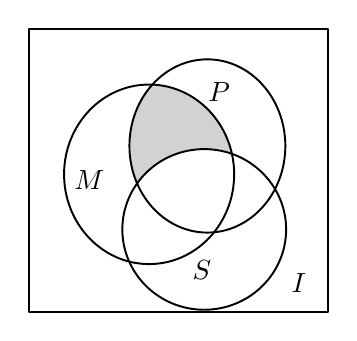
\begin{tikzpicture}[line join=round, line cap=round]
  % Shade M intersect P outside S.
  \begin{scope}
    \clip (-0.12,0.20) ellipse (1.08 and 1.14);
    \clip (0.62,0.56) ellipse (0.99 and 1.10);
    \fill[gray!35,even odd rule] (-1.70,-1.65) rectangle (2.30,2.10)
      (0.58,-0.50) ellipse (1.04 and 1.02);
  \end{scope}

  \draw[line width=0.7pt] (-1.65,-1.55) rectangle (2.15,2.05);
  \draw[line width=0.7pt] (-0.12,0.20) ellipse (1.08 and 1.14);
  \draw[line width=0.7pt] (0.62,0.56) ellipse (0.99 and 1.10);
  \draw[line width=0.7pt] (0.58,-0.50) ellipse (1.04 and 1.02);

  \node at (-0.88,0.13) {$M$};
  \node at (0.77,1.25) {$P$};
  \node at (0.55,-1.02) {$S$};
  \node at (1.78,-1.18) {$I$};
\end{tikzpicture}
\end{center}
\nopagebreak[4]
\end{question}
\begin{question}
\gkti{2}已知映射 $f:A\to B$，其中，集合 $A=\{-3,-2,-1,1,2,3,4\}$，集合 $B$ 中的元素都是 $A$ 中元素在映射 $f$ 下的象，且对任意的 $a\in A$，在 $B$ 中和它对应的元素是 $|a|$，则集合 $B$ 中元素的个数是

（A）4；（B）5；（C）6；（D）7。

\end{question}
\begin{question}
\gkti{3}若函数 $y=f(x)$ 的反函数是 $y=g(x)$，$f(a)=b$，$ab\ne0$，则 $g(b)$ 等于

（A）$a$；（B）$a^{-1}$；（C）$b$；（D）$b^{-1}$。

\end{question}
\begin{question}
\gkti{4}函数 $f(x)=M\sin(\omega x+\psi)$（$\omega>0$）在区间 $[a,b]$ 上是增函数，且 $f(a)=-M$，$f(b)=M$，则函数 $g(x)=M\cos(\omega x+\psi)$ 在 $[a,b]$ 上

（A）是增函数；（B）是减函数；（C）可以取得最大值 $M$；（D）可以取得最小值 $-M$。

\end{question}
\begin{question}
\gkti{5}若 $f(x)\sin x$ 是周期为 $\pi$ 的奇函数，则 $f(x)$ 可以是

（A）$\sin x$；（B）$\cos x$；（C）$\sin 2x$；（D）$\cos 2x$。

\end{question}
\begin{question}
\gkti{6}在极坐标系中，曲线 $\rho=4\sin\left(\theta-\dfrac\pi3\right)$ 关于

（A）直线 $\theta=\dfrac\pi3$ 轴对称；（B）直线 $\theta=\dfrac56\pi$ 轴对称；（C）点 $\left(2,\dfrac\pi3\right)$ 中心对称；（D）极点中心对称。

\end{question}
\begin{question}
\gkti{7}若干毫升水倒入底面半径为 2 cm 的圆柱形器皿中，量得水面的高度为 6 cm。若将这些水倒入轴截面是正三角形的倒圆锥形器皿中，则水面的高度是

（A）$6\sqrt3$ cm；（B）6 cm；（C）$2\sqrt[3]{18}$ cm；（D）$3\sqrt[3]{12}$ cm。

\end{question}
\begin{question}
\gkti{8}若 $(2x+\sqrt3)^3=a_0+a_1x+a_2x^2+a_3x^3$，则 $(a_0+a_2)^2-(a_1+a_3)^2$ 的值为

（A）$-1$；（B）1；（C）0；（D）2。

\end{question}
\begin{question}
\gkti{9}直线 $\sqrt3x+y-2\sqrt3=0$ 截圆 $x^2+y^2=4$ 得的劣弧所对的圆心角为

（A）$\dfrac\pi6$；（B）$\dfrac\pi4$；（C）$\dfrac\pi3$；（D）$\dfrac\pi2$。

\Needspace{0.4\textheight}
\end{question}
\begin{question}
\gkti{10}如图，在多面体 $ABCDEF$ 中，已知面 $ABCD$ 是边长为 3 的正方形，$EF\parallel AB$，$EF=\dfrac32$，$EF$ 与面 $AC$ 的距离为 2，则该多面体的体积为

（A）$\dfrac92$；（B）5；（C）6；（D）$\dfrac{15}{2}$。
\nopagebreak[4]
\begin{center}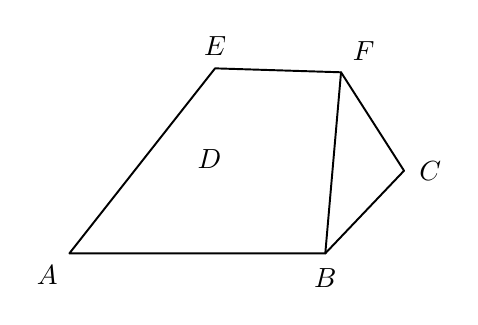
\begin{tikzpicture}[line join=round, line cap=round]
  \coordinate (A) at (0,0);
  \coordinate (B) at (3.25,0);
  \coordinate (C) at (4.25,1.05);
  \coordinate (E) at (1.85,2.35);
  \coordinate (F) at (3.45,2.30);

  \draw[line width=0.7pt] (A)--(B)--(C)--(F)--(E)--cycle;
  \draw[line width=0.7pt] (B)--(F);

  \node[below left=1pt] at (A) {$A$};
  \node[below=2pt] at (B) {$B$};
  \node[right=2pt] at (C) {$C$};
  \node[above=1pt] at (E) {$E$};
  \node[above right=1pt] at (F) {$F$};
  \node at (1.78,1.20) {$D$};
\end{tikzpicture}
\end{center}
\nopagebreak[4]
\end{question}
\begin{question}
\gkti{11}若 $\sin\alpha>\operatorname{tg}\alpha>\operatorname{ctg}\alpha$（$-\dfrac\pi2<\alpha<\dfrac\pi2$），则 $\alpha\in$

（A）$\left(-\dfrac\pi2,-\dfrac\pi4\right)$；（B）$\left(-\dfrac\pi4,0\right)$；（C）$\left(0,\dfrac\pi4\right)$；（D）$\left(\dfrac\pi4,\dfrac\pi2\right)$。

\end{question}
\begin{question}
\gkti{12}某电脑用户计划使用不超过 500 元的资金购买单价分别为 60 元、70 元的单片软件和盒装磁盘。根据需要，软件至少买 3 片，磁盘至少买 2 盒，则不同的选购方式共有

（A）5 种；（B）6 种；（C）7 种；（D）8 种。

\end{question}
\gkpart{第 II 卷　非选择题（共 90 分）}

\gksubpart{填空题（共 4 题，每题 4 分，共 16 分）}

\begin{question}
\gkti{13}设椭圆 $\dfrac{x^2}{a^2}+\dfrac{y^2}{b^2}=1$（$a>b>0$）的右焦点为 $F_1$，右准线为 $l_1$。若经过 $F$，且垂直于 $x$ 轴的弦长等于点 $F_1$ 到 $l_1$ 的距离，则椭圆的离心率为[原卷在此后重复/疑似错排：“的距离，则椭圆的离心率是”]\gkblank{}。

\end{question}
\begin{question}
\gkti{14}在一块并排 10 垄的田地中，选择 2 垄分别种植 $A,B$ 两种作物，每种作物种植一垄。为有利于作物生长，要求 $A,B$ 两种作物的间隔不小于 6 垄，则不同的选垄方法共有\gkblank{}种（用数字作答）。

\end{question}
\begin{question}
\gkti{15}若正数 $a,b$ 满足 $ab=a+b+3$，则 $ab$ 的取值范围是\gkblank{}。

\end{question}
\begin{question}
\gkti{16}$\alpha,\beta$ 是两个不同的平面，$m,n$ 是平面 $\alpha$ 及 $\beta$ 之外的两条不同直线。给出四个论断：

① $m\perp n$；　② $\alpha\perp\beta$；　③ $n\perp\beta$；　④ $m\perp\alpha$。

以其中三个论断作为条件，余下一个论断作为结论，写出你认为正确的一个命题：\gkblank{}。

\end{question}
\gksubpart{解答题（共 6 题，共 74 分）}

\begin{question}
\gkti{17}\textbf{（本小题满分 10 分）} 解方程 $\sqrt{3\lg x-2}-3\lg x+4=0$。

\end{question}
\begin{question}
\gkti{18}\textbf{（本小题满分 12 分）} 设复数 $z=3\cos\theta+i\cdot2\sin\theta$。求函数 $y=\operatorname{tg}(\theta-\arg z)$（$0<\theta<\dfrac\pi2$）的最大值以及对应的 $\theta$ 值。

\Needspace{0.4\textheight}
\end{question}
\begin{question}
\gkti{19}\textbf{（本小题满分 12 分）} 如图，已知正四棱柱 $ABCD-A_1B_1C_1D_1$，点 $E$ 在棱 $D_1D$ 上，截面 $EAC\parallel D_1B$，且面 $EAC$ 与底面 $ABCD$ 所成的角为 $45^\circ$，$AB=a$。

（Ⅰ）求截面 $EAC$ 的面积；

（Ⅱ）求异面直线 $A_1B_1$ 与 $AC$ 之间的距离；

（Ⅲ）求三棱锥 $B_1-EAC$ 的体积。
\nopagebreak[4]
\begin{center}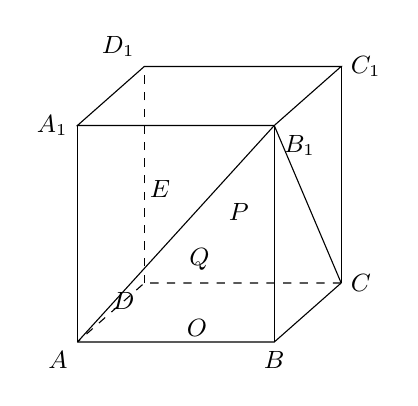
\begin{tikzpicture}[font=\small]
  \coordinate (A) at (0,0);
  \coordinate (B) at (2.5,0);
  \coordinate (C) at (3.35,0.75);
  \coordinate (D) at (0.85,0.75);
  \coordinate (A1) at (0,2.75);
  \coordinate (B1) at (2.5,2.75);
  \coordinate (C1) at (3.35,3.5);
  \coordinate (D1) at (0.85,3.5);
  \draw (A)--(B)--(C);
  \draw[dashed] (C)--(D)--(A);
  \draw (A)--(A1) (B)--(B1) (C)--(C1);
  \draw[dashed] (D)--(D1);
  \draw (A1)--(B1)--(C1)--(D1)--cycle;
  \draw (A)--(B1) (B1)--(C);
  \node at (1.05,1.95) {$E$};
  \node at (2.05,1.65) {$P$};
  \node at (1.55,1.05) {$Q$};
  \node at (1.52,0.18) {$O$};
  \node[below left] at (A) {$A$};
  \node[below] at (B) {$B$};
  \node[right] at (C) {$C$};
  \node[below left] at (D) {$D$};
  \node[left] at (A1) {$A_1$};
  \node[below right] at (B1) {$B_1$};
  \node[right] at (C1) {$C_1$};
  \node[above left] at (D1) {$D_1$};
\end{tikzpicture}
\end{center}
\nopagebreak[4]
\Needspace{0.4\textheight}
\end{question}
\begin{question}
\gkti{20}\textbf{（本小题满分 12 分）} 右图为一台冷轧机的示意图。冷轧机由若干对轧辊组成，带钢从一端输入，经过各对轧辊逐步减薄后输出。

（Ⅰ）输入带钢的厚度为 $\alpha$，输出带钢的厚度为 $\beta$，若每对轧辊的减薄率不超过 $r_0$。问冷轧机至少需要安装多少对轧辊？

（一对轧辊减薄率 $=\dfrac{\text{\text{输入该对的带钢厚度}}-\text{\text{从该对输出的带钢厚度}}}{\text{\text{输入该对的带钢厚度}}}$。）

（Ⅱ）已知一台冷轧机共有 4 对减薄率为 20\% 的轧辊，所有轧辊周长均为 1600 mm。若第 $\kappa$ 对轧辊有缺陷，每滚动一周在带钢上压出一个疵点，在冷轧机输出的带钢上，疵点的间距为 $L_\kappa$。为了便于检修，请计算 $L_1,L_2,L_3$ 并填入下表（轧钢过程中，带钢宽度不变，且不考虑损耗）。

\begin{center}
\begin{tabular}{lrrrr}
\toprule
轧辊序号 $\kappa$ & 1 & 2 & 3 & 4 \\
\midrule
疵点间距 $L_\kappa$（单位：mm） &  &  &  & 1600 \\
\bottomrule
\end{tabular}
\end{center}
\nopagebreak[4]
\begin{center}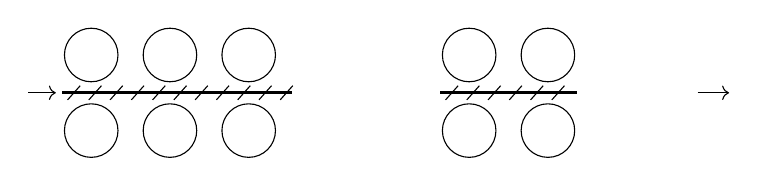
\begin{tikzpicture}[font=\small]
  \draw[->] (-0.35,0)--(0,0);
  \draw[->] (8.15,0)--(8.55,0);
  \foreach \x in {0.45,1.45,2.45} {
    \draw (\x,0.48) circle (0.34);
    \draw (\x,-0.48) circle (0.34);
  }
  \foreach \x in {5.25,6.25} {
    \draw (\x,0.48) circle (0.34);
    \draw (\x,-0.48) circle (0.34);
  }
  \draw[line width=1.1pt] (0.08,0)--(3.0,0);
  \draw[line width=1.1pt] (4.88,0)--(6.62,0);
  \foreach \x in {0.15,0.42,...,2.88} {
    \draw (\x,-0.09)--++(0.16,0.18);
  }
  \foreach \x in {4.95,5.22,...,6.5} {
    \draw (\x,-0.09)--++(0.16,0.18);
  }
\end{tikzpicture}
\end{center}
\nopagebreak[4]
\end{question}
\begin{question}
\gkti{21}\textbf{（本小题满分 14 分）} 已知函数 $y=f(x)$ 的图像是自原点出发的一条折线。当 $n\leq y\leq n+1$（$n=0,1,2,\ldots$）时，该图像是斜率为 $b^n$ 的线段（其中正常数 $b\ne1$）。设数列 $\{x_n\}$ 由[原卷字面为 $x(x_n)=n$，符号可辨但原意不明]（$n=1,2,\ldots$）定义。

（Ⅰ）求[原卷此处列式可见为 $x_1,x_2x$ 和 $x_n$，待复核]的表达式；

（Ⅱ）计算 $\displaystyle\lim_{n\to\infty}x_n$；

（Ⅲ）求 $f(x)$ 的表达式，并写出其定义域。

\Needspace{0.4\textheight}
\end{question}
\begingroup
\renewenvironment{question}{\Needspace{0.05\textheight}}{}
\begin{question}
\gkti{22}\textbf{（本小题满分 14 分）} 如图，给出定点 $A(a,0)$（$a>0$，$a\ne1$）和直线 $l:x=-1$。$B$ 是直线 $l$ 上的动点，$\angle BOA$ 的角平分线交 $AB$ 于点 $C$。求点 $C$ 的轨迹方程，并讨论方程表示的曲线类型与 $a$ 值的关系。
\nopagebreak[4]
\begin{center}\begin{tikzpicture}[font=\small]
  \draw[->] (-1.35,0)--(3.1,0) node[right] {$x$};
  \draw[->] (0,-1.05)--(0,2.65) node[above] {$y$};
  \draw (-0.82,-1.05)--(-0.82,2.35) node[above] {$l$};
  \coordinate (O) at (0,0);
  \coordinate (A) at (2.55,0);
  \coordinate (B) at (-0.82,1.55);
  \coordinate (C) at (0.86,0.78);
  \draw (B)--(A);
  \draw (B)--(O);
  \draw (O)--(C);
  \fill (O) circle (0.7pt);
  \node[below left] at (O) {$O$};
  \node[below] at (A) {$A$};
  \node[left] at (B) {$B$};
  \node[above right] at (C) {$C$};
\end{tikzpicture}
\end{center}
\nopagebreak[4]

\end{question}
\endgroup
\clearpage
\pdfbookmark[1]{参考答案与详细解析}{sec:s}
\Needspace{8\baselineskip}
\begin{center}{\Large\bfseries 参考答案与详细解析}\end{center}
\medskip
% answers.tex —— 1999 年·普通高等学校招生全国统一考试·广东卷 · 参考答案与详细解析片段
% 由 tools/generate_projects.py 依来源总账自 1999/1999_数学真题_广东_试题.md + 1999/1999_数学真题_广东_解析正文.md + 1999/1999_数学真题_广东_答案要点.md 生成，勿手改（改源 MD 后重跑）


\begin{gktip}
本文的推导按固定扫描件题面进行。来源身份及卷内“答案要点及评分标准”的发布身份未核。Q10、Q13、Q21 的题意存在未决点，以下保留不确定性。
\end{gktip}

\begin{answer}
\gksolhead{1}{}

\textbf{题目}：

如图，$I$ 是全集，$M,P,S$ 是 $I$ 的 3 个子集，则阴影部分所表示的集合是

（A）$(M\cap P)\cap S$；（B）$(M\cap P)\cup S$；（C）$(M\cap P)\cap\overline S$；（D）$(M\cap P)\cup\overline S$。
\nopagebreak[4]
\begin{center}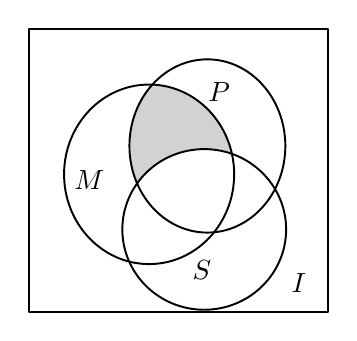
\begin{tikzpicture}[line join=round, line cap=round]
  % Shade M intersect P outside S.
  \begin{scope}
    \clip (-0.12,0.20) ellipse (1.08 and 1.14);
    \clip (0.62,0.56) ellipse (0.99 and 1.10);
    \fill[gray!35,even odd rule] (-1.70,-1.65) rectangle (2.30,2.10)
      (0.58,-0.50) ellipse (1.04 and 1.02);
  \end{scope}

  \draw[line width=0.7pt] (-1.65,-1.55) rectangle (2.15,2.05);
  \draw[line width=0.7pt] (-0.12,0.20) ellipse (1.08 and 1.14);
  \draw[line width=0.7pt] (0.62,0.56) ellipse (0.99 and 1.10);
  \draw[line width=0.7pt] (0.58,-0.50) ellipse (1.04 and 1.02);

  \node at (-0.88,0.13) {$M$};
  \node at (0.77,1.25) {$P$};
  \node at (0.55,-1.02) {$S$};
  \node at (1.78,-1.18) {$I$};
\end{tikzpicture}
\end{center}
\nopagebreak[4]
\Needspace{4\baselineskip}
\textbf{解析}

阴影区域位于 $M$ 与 $P$ 的公共部分，同时在 $S$ 外，因此对应 $(M\cap P)\cap\overline S$，选 C。

\gkanswer{答案：C。}

\end{answer}
\begin{answer}
\gksolhead{2}{}

\textbf{题目}：

已知映射 $f:A\to B$，其中，集合 $A=\{-3,-2,-1,1,2,3,4\}$，集合 $B$ 中的元素都是 $A$ 中元素在映射 $f$ 下的象，且对任意的 $a\in A$，在 $B$ 中和它对应的元素是 $|a|$，则集合 $B$ 中元素的个数是

（A）4；（B）5；（C）6；（D）7。

\Needspace{4\baselineskip}
\textbf{解析}

$B$ 是 $A$ 中各元素绝对值组成的集合：$B=\{1,2,3,4\}$，共有 4 个元素，选 A。

\gkanswer{答案：A。}

\end{answer}
\begin{answer}
\gksolhead{3}{}

\textbf{题目}：

若函数 $y=f(x)$ 的反函数是 $y=g(x)$，$f(a)=b$，$ab\ne0$，则 $g(b)$ 等于

（A）$a$；（B）$a^{-1}$；（C）$b$；（D）$b^{-1}$。

\Needspace{4\baselineskip}
\textbf{解析}

反函数 $g$ 满足 $g(f(a))=a$。由 $f(a)=b$ 得 $g(b)=a$，选 A。

\gkanswer{答案：A。}

\end{answer}
\begin{answer}
\gksolhead{4}{}

\textbf{题目}：

函数 $f(x)=M\sin(\omega x+\psi)$（$\omega>0$）在区间 $[a,b]$ 上是增函数，且 $f(a)=-M$，$f(b)=M$，则函数 $g(x)=M\cos(\omega x+\psi)$ 在 $[a,b]$ 上

（A）是增函数；（B）是减函数；（C）可以取得最大值 $M$；（D）可以取得最小值 $-M$。

\Needspace{4\baselineskip}
\textbf{解析}

$f$ 在区间上从 $-M$ 增至 $M$，正弦相位沿单调上升的一段半周期变化。相位经过 $\pi/2$（模 $2\pi$）时，$g=M\cos(\omega x+\psi)$ 取得最大值 $M$，选 C。

\gkanswer{答案：C。}

\end{answer}
\begin{answer}
\gksolhead{5}{}

\textbf{题目}：

若 $f(x)\sin x$ 是周期为 $\pi$ 的奇函数，则 $f(x)$ 可以是

（A）$\sin x$；（B）$\cos x$；（C）$\sin 2x$；（D）$\cos 2x$。

\Needspace{4\baselineskip}
\textbf{解析}

取 $f(x)=\cos x$，则 $f(x)\sin x=\frac12\sin2x$，是奇函数，且周期为 $\pi$，选 B。

\gkanswer{答案：B。}

\end{answer}
\begin{answer}
\gksolhead{6}{}

\textbf{题目}：

在极坐标系中，曲线 $\rho=4\sin\left(\theta-\dfrac\pi3\right)$ 关于

（A）直线 $\theta=\dfrac\pi3$ 轴对称；（B）直线 $\theta=\dfrac56\pi$ 轴对称；（C）点 $\left(2,\dfrac\pi3\right)$ 中心对称；（D）极点中心对称。

\Needspace{4\baselineskip}
\textbf{解析}

\Needspace{5\baselineskip}
由 $\rho=4\sin(\theta-\pi/3)$ 及 $x=\rho\cos\theta$、$y=\rho\sin\theta$，得

\nopagebreak[4]
\[
x^2+y^2=2y-2\sqrt3x,
\]

即圆心为 $(-\sqrt3,1)$ 的圆。圆心所在射线的极角为 $5\pi/6$，该圆关于过原点与圆心的直线对称，选 B。

\gkanswer{答案：B。}

\end{answer}
\begin{answer}
\gksolhead{7}{}

\textbf{题目}：

若干毫升水倒入底面半径为 2 cm 的圆柱形器皿中，量得水面的高度为 6 cm。若将这些水倒入轴截面是正三角形的倒圆锥形器皿中，则水面的高度是

（A）$6\sqrt3$ cm；（B）6 cm；（C）$2\sqrt[3]{18}$ cm；（D）$3\sqrt[3]{12}$ cm。

\Needspace{4\baselineskip}
\textbf{解析}

水的体积为 $\pi\cdot2^2\cdot6=24\pi$。倒圆锥的轴截面为正三角形，故水面半径 $r=h/\sqrt3$，其容积为 $\frac13\pi r^2h=\pi h^3/9$。令其等于 $24\pi$，得 $h=6$ cm，选 B。

\gkanswer{答案：B。}

\end{answer}
\begin{answer}
\gksolhead{8}{}

\textbf{题目}：

若 $(2x+\sqrt3)^3=a_0+a_1x+a_2x^2+a_3x^3$，则 $(a_0+a_2)^2-(a_1+a_3)^2$ 的值为

（A）$-1$；（B）1；（C）0；（D）2。

\Needspace{4\baselineskip}
\textbf{解析}

\Needspace{5\baselineskip}
展开得 $a_0=3\sqrt3$、$a_1=18$、$a_2=12\sqrt3$、$a_3=8$。因此

\nopagebreak[4]
\[
(a_0+a_2)^2-(a_1+a_3)^2=(15\sqrt3)^2-26^2=-1,
\]

选 A。

\gkanswer{答案：A。}

\end{answer}
\begin{answer}
\gksolhead{9}{}

\textbf{题目}：

直线 $\sqrt3x+y-2\sqrt3=0$ 截圆 $x^2+y^2=4$ 得的劣弧所对的圆心角为

（A）$\dfrac\pi6$；（B）$\dfrac\pi4$；（C）$\dfrac\pi3$；（D）$\dfrac\pi2$。

\Needspace{4\baselineskip}
\textbf{解析}

\Needspace{5\baselineskip}
圆心到直线的距离为 $|{-2\sqrt3}|/\sqrt{3+1}=\sqrt3$，圆半径为 2。劣弧所对圆心角为

\nopagebreak[4]
\[
2\arccos\frac{\sqrt3}{2}=\frac\pi3,
\]

选 C。

\gkanswer{答案：C。}

\end{answer}
\begin{answer}
\gksolhead{10}{}

\textbf{题目}：

如图，在多面体 $ABCDEF$ 中，已知面 $ABCD$ 是边长为 3 的正方形，$EF\parallel AB$，$EF=\dfrac32$，$EF$ 与面 $AC$ 的距离为 2，则该多面体的体积为

（A）$\dfrac92$；（B）5；（C）6；（D）$\dfrac{15}{2}$。
\nopagebreak[4]
\begin{center}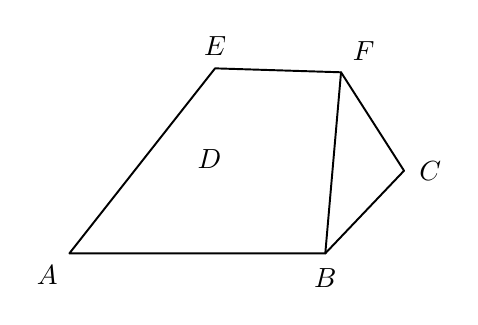
\begin{tikzpicture}[line join=round, line cap=round]
  \coordinate (A) at (0,0);
  \coordinate (B) at (3.25,0);
  \coordinate (C) at (4.25,1.05);
  \coordinate (E) at (1.85,2.35);
  \coordinate (F) at (3.45,2.30);

  \draw[line width=0.7pt] (A)--(B)--(C)--(F)--(E)--cycle;
  \draw[line width=0.7pt] (B)--(F);

  \node[below left=1pt] at (A) {$A$};
  \node[below=2pt] at (B) {$B$};
  \node[right=2pt] at (C) {$C$};
  \node[above=1pt] at (E) {$E$};
  \node[above right=1pt] at (F) {$F$};
  \node at (1.78,1.20) {$D$};
\end{tikzpicture}
\end{center}
\nopagebreak[4]
\Needspace{4\baselineskip}
\textbf{解析}

\textbf{未决说明。} 固定扫描件 A 型答案栏印为 D，但原题“$EF$ 与面 $AC$ 的距离”所指平面记号不完整或有歧义。现有文字和示意图不足以独立确认体积条件；在取得可核验的同版补源或明确勘误前，不据答案栏强行给出解析。

\gkanswer{答案：U/PENDING}

\end{answer}
\begin{answer}
\gksolhead{11}{}

\textbf{题目}：

若 $\sin\alpha>\operatorname{tg}\alpha>\operatorname{ctg}\alpha$（$-\dfrac\pi2<\alpha<\dfrac\pi2$），则 $\alpha\in$

（A）$\left(-\dfrac\pi2,-\dfrac\pi4\right)$；（B）$\left(-\dfrac\pi4,0\right)$；（C）$\left(0,\dfrac\pi4\right)$；（D）$\left(\dfrac\pi4,\dfrac\pi2\right)$。

\Needspace{4\baselineskip}
\textbf{解析}

\Needspace{5\baselineskip}
在 $-\pi/4<\alpha<0$ 时，$\sin\alpha$、$\tan\alpha$、$\cot\alpha$ 均为负，且

\nopagebreak[4]
\[
\sin\alpha>\tan\alpha>\cot\alpha.
\]

其他区间不满足三者的该顺序，故选 B。

\gkanswer{答案：B。}

\end{answer}
\begin{answer}
\gksolhead{12}{}

\textbf{题目}：

某电脑用户计划使用不超过 500 元的资金购买单价分别为 60 元、70 元的单片软件和盒装磁盘。根据需要，软件至少买 3 片，磁盘至少买 2 盒，则不同的选购方式共有

（A）5 种；（B）6 种；（C）7 种；（D）8 种。

\Needspace{4\baselineskip}
\textbf{解析}

设买软件 $x$ 片、磁盘 $y$ 盒，则 $x\ge3$、$y\ge2$ 且 $60x+70y\le500$。当 $y=2$ 时有 $x=3,4,5,6$ 共 4 种；$y=3$ 时有 $x=3,4$ 共 2 种；$y=4$ 时有 $x=3$ 共 1 种，总计 7 种，选 C。

\gkanswer{答案：C。}

\end{answer}
\begin{answer}
\gksolhead{13}{}

\textbf{题目}：

设椭圆 $\dfrac{x^2}{a^2}+\dfrac{y^2}{b^2}=1$（$a>b>0$）的右焦点为 $F_1$，右准线为 $l_1$。若经过 $F$，且垂直于 $x$ 轴的弦长等于点 $F_1$ 到 $l_1$ 的距离，则椭圆的离心率为[原卷在此后重复/疑似错排：“的距离，则椭圆的离心率是”]\gkblank{}。

\Needspace{4\baselineskip}
\textbf{解析}

\textbf{条件推导：} 若首处 $F$ 本意为已定义的右焦点 $F_1$，则过焦点的竖弦长为 $2b^2/a$，右焦点到右准线的距离为 $a^2/c-c=b^2/c$。令二者相等并设 $e=c/a$，约去 $b^2>0$ 得 $2/a=1/c$，所以 $e=1/2$。但原件明确出现 $F/F_1$ 冲突且题干有重复错排，故本题暂不将该数值认定为无条件答案。

\gkanswer{答案：条件答案 $e=\dfrac12$；原题按可见字面未决。}

\end{answer}
\begin{answer}
\gksolhead{14}{}

\textbf{题目}：

在一块并排 10 垄的田地中，选择 2 垄分别种植 $A,B$ 两种作物，每种作物种植一垄。为有利于作物生长，要求 $A,B$ 两种作物的间隔不小于 6 垄，则不同的选垄方法共有\gkblank{}种（用数字作答）。

\Needspace{4\baselineskip}
\textbf{解析}

“间隔不小于 6 垄”按两种作物之间至少空 6 垄理解，则两垄序号差至少为 7。可选无序位置对为 $(1,8)$、$(1,9)$、$(1,10)$、$(2,9)$、$(2,10)$、$(3,10)$，共 6 对。A、B 两种作物可互换位置，故共有 $6\times2=12$ 种。

\gkanswer{答案：12。}

\end{answer}
\begin{answer}
\gksolhead{15}{}

\textbf{题目}：

若正数 $a,b$ 满足 $ab=a+b+3$，则 $ab$ 的取值范围是\gkblank{}。

\Needspace{4\baselineskip}
\textbf{解析}

令 $p=ab$。由 $ab=a+b+3$ 得 $a+b=p-3$。因 $a,b>0$，有 $(a+b)^2\ge4ab$，即 $(p-3)^2\ge4p$，从而 $(p-1)(p-9)\ge0$。又 $p=a+b+3>3$，所以 $p\ge9$；等号在 $a=b=3$ 时成立，故范围为 $[9,+\infty)$。

\gkanswer{答案：$[9,+\infty)$。}

\end{answer}
\begin{answer}
\gksolhead{16}{}

\textbf{题目}：

$\alpha,\beta$ 是两个不同的平面，$m,n$ 是平面 $\alpha$ 及 $\beta$ 之外的两条不同直线。给出四个论断：

① $m\perp n$；　② $\alpha\perp\beta$；　③ $n\perp\beta$；　④ $m\perp\alpha$。

以其中三个论断作为条件，余下一个论断作为结论，写出你认为正确的一个命题：\gkblank{}。

\Needspace{4\baselineskip}
\textbf{解析}

若 $m\perp\alpha$、$n\perp\beta$ 且 $\alpha\perp\beta$，则 $n$ 平行于平面 $\alpha$，而 $m\perp\alpha$，所以 $m\perp n$。另若 $m\perp n$、$m\perp\alpha$ 且 $n\perp\beta$，则 $m$ 平行于平面 $\beta$；结合 $m\perp\alpha$ 得 $\alpha\perp\beta$。两种均为成立命题。

\gkanswer{答案：$m\perp\alpha,\ n\perp\beta,\ \alpha\perp\beta\Rightarrow m\perp n$；或 $m\perp n,\ m\perp\alpha,\ n\perp\beta\Rightarrow\alpha\perp\beta$。}

\end{answer}
\begin{answer}
\gksolhead{17}{}

\textbf{题目}（本小题满分 10 分）：

解方程 $\sqrt{3\lg x-2}-3\lg x+4=0$。

\Needspace{4\baselineskip}
\textbf{解析}

令 $t=3\lg x-2$，根式要求 $t\ge0$。原方程化为 $\sqrt t-t+2=0$。令 $u=\sqrt t\ge0$，则 $u^2-u-2=0$，取 $u=2$，得 $t=4$、$\lg x=2$，所以 $x=100$。

\gkanswer{答案：$x=100$。}

\end{answer}
\begin{answer}
\gksolhead{18}{}

\textbf{题目}（本小题满分 12 分）：

设复数 $z=3\cos\theta+i\cdot2\sin\theta$。求函数 $y=\operatorname{tg}(\theta-\arg z)$（$0<\theta<\dfrac\pi2$）的最大值以及对应的 $\theta$ 值。

\Needspace{4\baselineskip}
\textbf{解析}

\Needspace{5\baselineskip}
由 $z=3\cos\theta+2i\sin\theta$，可得

\nopagebreak[4]
\[
\tan(\theta-\arg z)=\frac{\sin\theta\cos\theta}{3\cos^2\theta+2\sin^2\theta}.
\]

令 $t=\tan\theta>0$，右式为 $t/(3+2t^2)$，其导数为 $(3-2t^2)/(3+2t^2)^2$。故在 $t=\sqrt{3/2}$ 处取最大值 $\sqrt6/12$，对应 $\theta=\arctan\sqrt{3/2}$。

\gkanswer{答案：最大值 $\dfrac{\sqrt6}{12}$，对应 $\theta=\arctan\sqrt{\dfrac32}$。}

\end{answer}
\begin{answer}
\gksolhead{19}{}

\textbf{题目}（本小题满分 12 分）：

如图，已知正四棱柱 $ABCD-A_1B_1C_1D_1$，点 $E$ 在棱 $D_1D$ 上，截面 $EAC\parallel D_1B$，且面 $EAC$ 与底面 $ABCD$ 所成的角为 $45^\circ$，$AB=a$。

（Ⅰ）求截面 $EAC$ 的面积；

（Ⅱ）求异面直线 $A_1B_1$ 与 $AC$ 之间的距离；

（Ⅲ）求三棱锥 $B_1-EAC$ 的体积。
\nopagebreak[4]
\begin{center}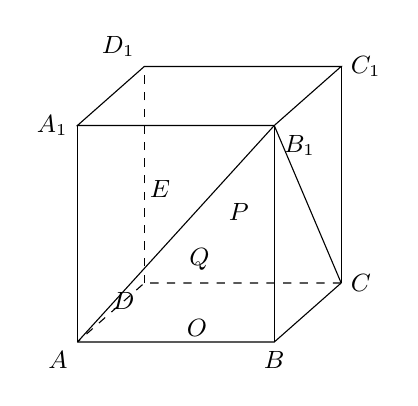
\begin{tikzpicture}[font=\small]
  \coordinate (A) at (0,0);
  \coordinate (B) at (2.5,0);
  \coordinate (C) at (3.35,0.75);
  \coordinate (D) at (0.85,0.75);
  \coordinate (A1) at (0,2.75);
  \coordinate (B1) at (2.5,2.75);
  \coordinate (C1) at (3.35,3.5);
  \coordinate (D1) at (0.85,3.5);
  \draw (A)--(B)--(C);
  \draw[dashed] (C)--(D)--(A);
  \draw (A)--(A1) (B)--(B1) (C)--(C1);
  \draw[dashed] (D)--(D1);
  \draw (A1)--(B1)--(C1)--(D1)--cycle;
  \draw (A)--(B1) (B1)--(C);
  \node at (1.05,1.95) {$E$};
  \node at (2.05,1.65) {$P$};
  \node at (1.55,1.05) {$Q$};
  \node at (1.52,0.18) {$O$};
  \node[below left] at (A) {$A$};
  \node[below] at (B) {$B$};
  \node[right] at (C) {$C$};
  \node[below left] at (D) {$D$};
  \node[left] at (A1) {$A_1$};
  \node[below right] at (B1) {$B_1$};
  \node[right] at (C1) {$C_1$};
  \node[above left] at (D1) {$D_1$};
\end{tikzpicture}
\end{center}
\nopagebreak[4]
\Needspace{4\baselineskip}
\textbf{解析}

设底面顶点坐标为 $A(0,0,0)$、$B(a,0,0)$、$C(a,a,0)$、$D(0,a,0)$，令 $E=(0,a,e)$、$D_1=(0,a,h)$。截面 $EAC$ 可写为 $ex-ey+az=0$。它与底面的夹角为 $45^\circ$，故 $\tan45^\circ=\sqrt2e/a$，从而 $DE=e=a/\sqrt2$。又 $D_1B$ 的方向向量为 $(a,-a,-h)$；该直线平行于平面 $EAC$，代入平面法向量 $(e,-e,a)$ 得 $2ae-ah=0$，所以棱柱高 $DD_1=h=2e=\sqrt2a$。

\Needspace{5\baselineskip}
点 $E$ 到对角线 $AC$ 的距离为 $a$，于是 $S_{EAC}=\frac12(a\sqrt2)a=a^2/\sqrt2$。$A_1A$ 垂直于 $A_1B_1$ 和 $AC$，故两异面直线的距离为 $AA_1=h=\sqrt2a$。点 $B_1$ 到平面 $EAC$ 的距离为 $3a/2$，所以三棱锥体积为

\nopagebreak[4]
\[
V=\frac13\cdot\frac{a^2}{\sqrt2}\cdot\frac{3a}{2}=\frac{a^3}{2\sqrt2}.
\]

\gkanswer{答案：$\dfrac{a^2}{\sqrt2}$；$\sqrt2a$；$\dfrac{a^3}{2\sqrt2}$。}

\end{answer}
\begin{answer}
\gksolhead{20}{}

\textbf{题目}（本小题满分 12 分）：

右图为一台冷轧机的示意图。冷轧机由若干对轧辊组成，带钢从一端输入，经过各对轧辊逐步减薄后输出。

（Ⅰ）输入带钢的厚度为 $\alpha$，输出带钢的厚度为 $\beta$，若每对轧辊的减薄率不超过 $r_0$。问冷轧机至少需要安装多少对轧辊？

（一对轧辊减薄率 $=\dfrac{\text{\text{输入该对的带钢厚度}}-\text{\text{从该对输出的带钢厚度}}}{\text{\text{输入该对的带钢厚度}}}$。）

（Ⅱ）已知一台冷轧机共有 4 对减薄率为 20\% 的轧辊，所有轧辊周长均为 1600 mm。若第 $\kappa$ 对轧辊有缺陷，每滚动一周在带钢上压出一个疵点，在冷轧机输出的带钢上，疵点的间距为 $L_\kappa$。为了便于检修，请计算 $L_1,L_2,L_3$ 并填入下表（轧钢过程中，带钢宽度不变，且不考虑损耗）。

\begin{center}
\begin{tabular}{lrrrr}
\toprule
轧辊序号 $\kappa$ & 1 & 2 & 3 & 4 \\
\midrule
疵点间距 $L_\kappa$（单位：mm） &  &  &  & 1600 \\
\bottomrule
\end{tabular}
\end{center}
\nopagebreak[4]
\begin{center}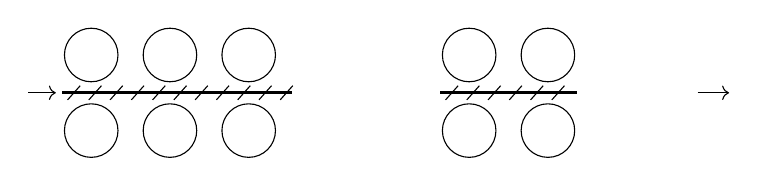
\begin{tikzpicture}[font=\small]
  \draw[->] (-0.35,0)--(0,0);
  \draw[->] (8.15,0)--(8.55,0);
  \foreach \x in {0.45,1.45,2.45} {
    \draw (\x,0.48) circle (0.34);
    \draw (\x,-0.48) circle (0.34);
  }
  \foreach \x in {5.25,6.25} {
    \draw (\x,0.48) circle (0.34);
    \draw (\x,-0.48) circle (0.34);
  }
  \draw[line width=1.1pt] (0.08,0)--(3.0,0);
  \draw[line width=1.1pt] (4.88,0)--(6.62,0);
  \foreach \x in {0.15,0.42,...,2.88} {
    \draw (\x,-0.09)--++(0.16,0.18);
  }
  \foreach \x in {4.95,5.22,...,6.5} {
    \draw (\x,-0.09)--++(0.16,0.18);
  }
\end{tikzpicture}
\end{center}
\nopagebreak[4]
\Needspace{4\baselineskip}
\textbf{解析}

\Needspace{5\baselineskip}
（Ⅰ）经过 $n$ 对轧辊后厚度至多为 $\alpha(1-r_0)^n$。要求不超过 $\beta$，故

\nopagebreak[4]
\[
n\ge\frac{\lg(\beta/\alpha)}{\lg(1-r_0)}.
\]

在 $0<\beta<\alpha$、$0<r_0<1$ 时，最少对数为该商向上取整。

（Ⅱ）带钢宽度不变且不计损耗，体积守恒，因此每道减薄 20\% 后，带钢长度及同一疵点间距放大 $1/0.8=1.25$ 倍。从第 $k$ 对轧辊到出口还经过 $4-k$ 道，故 $L_k=1600(1.25)^{4-k}$ mm。于是 $L_1=3125$ mm、$L_2=2500$ mm、$L_3=2000$ mm。

\gkanswer{答案：当 $0<\beta<\alpha$、$0<r_0<1$ 时，至少 $\left\lceil\dfrac{\lg(\beta/\alpha)}{\lg(1-r_0)}\right\rceil$ 对；$L_1=3125\ \mathrm{mm}$，$L_2=2500\ \mathrm{mm}$，$L_3=2000\ \mathrm{mm}$。}

\end{answer}
\begin{answer}
\gksolhead{21}{}

\textbf{题目}（本小题满分 14 分）：

已知函数 $y=f(x)$ 的图像是自原点出发的一条折线。当 $n\leq y\leq n+1$（$n=0,1,2,\ldots$）时，该图像是斜率为 $b^n$ 的线段（其中正常数 $b\ne1$）。设数列 $\{x_n\}$ 由[原卷字面为 $x(x_n)=n$，符号可辨但原意不明]（$n=1,2,\ldots$）定义。

（Ⅰ）求[原卷此处列式可见为 $x_1,x_2x$ 和 $x_n$，待复核]的表达式；

（Ⅱ）计算 $\displaystyle\lim_{n\to\infty}x_n$；

（Ⅲ）求 $f(x)$ 的表达式，并写出其定义域。

\Needspace{4\baselineskip}
\textbf{解析}

\Needspace{5\baselineskip}
\textbf{条件推导：} 若原定义本意为 $f(x_n)=n$，且 $x_0=0$，由于第 $n$ 段斜率为 $b^n$，每段的水平长度为 $b^{-n}$，故

\nopagebreak[4]
\[
x_n=\sum_{k=0}^{n-1}b^{-k}=\frac{1-b^{-n}}{1-b^{-1}}.
\]

当 $b>1$ 时，$x_n\to b/(b-1)$；当 $0<b<1$ 时，$x_n\to+\infty$。在 $[x_n,x_{n+1}]$ 上，折线可写为 $f(x)=n+b^n(x-x_n)$。因此条件解释下，$b>1$ 时定义域为 $[0,b/(b-1))$，$0<b<1$ 时定义域为 $[0,+\infty)$。但扫描件字面为 $x(x_n)=n$，且（Ⅰ）列式字样异常，以上只作为条件解释，不替代原题的未决文字。

\gkanswer{答案：条件性结论：若原定义本意为 $f(x_n)=n$，则（Ⅰ）$x_n=\sum_{k=0}^{n-1}b^{-k}=\dfrac{1-b^{-n}}{1-b^{-1}}$；（Ⅱ）$b>1$ 时极限为 $\dfrac{b}{b-1}$，$0<b<1$ 时极限为 $+\infty$；（Ⅲ）在 $[x_n,x_{n+1}]$ 上 $f(x)=n+b^n(x-x_n)$，定义域分别为 $[0,\dfrac{b}{b-1})$ 与 $[0,+\infty)$。原页字面为 $x(x_n)=n$ 且小问（Ⅰ）列式异常，因此以上不是无条件答案。}

\end{answer}
\begin{answer}
\gksolhead{22}{}

\textbf{题目}（本小题满分 14 分）：

如图，给出定点 $A(a,0)$（$a>0$，$a\ne1$）和直线 $l:x=-1$。$B$ 是直线 $l$ 上的动点，$\angle BOA$ 的角平分线交 $AB$ 于点 $C$。求点 $C$ 的轨迹方程，并讨论方程表示的曲线类型与 $a$ 值的关系。
\nopagebreak[4]
\begin{center}\begin{tikzpicture}[font=\small]
  \draw[->] (-1.35,0)--(3.1,0) node[right] {$x$};
  \draw[->] (0,-1.05)--(0,2.65) node[above] {$y$};
  \draw (-0.82,-1.05)--(-0.82,2.35) node[above] {$l$};
  \coordinate (O) at (0,0);
  \coordinate (A) at (2.55,0);
  \coordinate (B) at (-0.82,1.55);
  \coordinate (C) at (0.86,0.78);
  \draw (B)--(A);
  \draw (B)--(O);
  \draw (O)--(C);
  \fill (O) circle (0.7pt);
  \node[below left] at (O) {$O$};
  \node[below] at (A) {$A$};
  \node[left] at (B) {$B$};
  \node[above right] at (C) {$C$};
\end{tikzpicture}
\end{center}
\nopagebreak[4]
\Needspace{4\baselineskip}
\textbf{解析}

\Needspace{5\baselineskip}
按图示取 $\angle BOA$ 的内角平分线。由角平分线定理，$C\in AB$ 且 $AC/CB=AO/OB=a/|OB|$。设 $B=(-1,t)$，将 $C$ 写成 $A$、$B$ 的内分点坐标，并消去参数 $t$，可得

\nopagebreak[4]
\[
(1-a)x^2-2ax+(a+1)y^2=0.
\]

还需满足点在图示线段上的范围 $0\le x<a$。当 $0<a<1$ 时二次项同号，方程表示椭圆；当 $a>1$ 时二次项异号，表示双曲线，实际轨迹为符合上述范围的部分。

\gkanswer{答案：$(1-a)x^2-2ax+(a+1)y^2=0$，实际轨迹取 $0\leq x<a$；$0<a<1$ 时为椭圆，$a>1$ 时为双曲线的相应部分。}

\end{answer}
\end{document}
